\section{Анализ литературно патентных исследований}

% В данном разделе будет приведена информация про то что именно из
% себя представляет разрабатываемое устройство, а именно то,
% что оно является полётным контроллером.

% Также пять патентов схожих по параметрам
% устройств, выполняющих функции полётных контроллеров.

\subsection{Обзор методов 
  и средств управления  двигателями 
  мультироторных беспилотных летательных аппаратов}

В типичной системе контроля полета
мультироторного летательного аппарата
пять параметров подлежат отслеживанию: длина четырех управляющих
сервоприводами импульсов, которые контролируют тягу, крен, тангаж и
рысканье, и напряжение питания.

Управление скоростью вращения винтов квадрокоптера осуществляется
изменением уровня управляющих напряжений (или скважностью, если
управляющий сигнал широтно-импульсный). Как правило, двигатели
квадрокоптера — это двигатели постоянного тока, обладающие своей
динамикой ~\cite{liisuho}.
% % Лысухо Г.В., Масленников А.Л. Квадрокоптер: динамика и
% управление. Политехнический молодежный журнал, 2020, №
% 05(46). http://dx.doi.org/10.18698/2541-8009-2020-5-604


Наиболее часто в квадрокоптерах применяют бесколлекторные двигатели,
якорь которых представляет собой набор неодимовых магнитов, а статор
состоит из обмотки возбуждения, на который подается управляющее
напряжение. В отличие от коллекторных двигателей, где якорь вращается
внутри статора, у бесколлекторных якорь вращается постоянного тока
вокруг статора, который находится внутри~\cite{Solodovnikov1976}.
% Солодовников В.В., ред. Устройства и элементы систем автоматического
% регулирования. Техническая кибернетика. Кн. 3. Исполнительные
% устройства и сервомеха- низмы. М., Машиностроение, 1976.

Малогабаритные быстродействующие сервоприводы применяются в
современных высокоточных системах управления подвижными объектами:
рулевыми системами летательных аппаратов, автоматическими
манипуляторами, роботами с подвижными элементами конструкции и
др~\cite{dyakovSUBSTANTIATIONRELIABILITYSERVOMOTORS2023}.

Под сервоприводом в данной работе подразумевается вращающийся привод,
управляющий широтно-импульсной модуляцией, который за счёт обратной
связи позволяет точно контролировать вал сервопривода, поворачивая его
на заданный угол или поддерживая определенную скорость или ускорение.

Говоря кратко, разрабатываемое изделие, можно назвать одним
общепринятым словом — полётный контроллер.

Полётный контроллер выполнен в виде платы, на которую, с помощью
монтажа в отверстия помещаются компоненты. Такой способ монтажа выбран
для того, чтобы облегчить сборку данной схемы, установку и смену
тестируемых компонентов или незначительного изменения схемы,
необходимого для взаимодействия с определенными компонентами, а также
возможный ремонт.


\subsection{Анализ патентных исследований}

По своему характеру и содержанию патентные исследования относятся к
прикладным научно-исследовательским работам и являются неотъемлемой
составной частью обоснования принимаемых хозяйствующими субъектами
решений народнохозяйственных задач, связанных с созданием,
производством, реализацией, совершенствованием, использованием,
ремонтом и снятием с производства
объектов хозяйственной деятельности ~\cite{GOST-R-15.011-96}.

В ~\cite{US10144527B2} представлен полётный контроллер, который
включает в себя отдельный вход для сигнала поступающего с электронного
контроллера скорости. А также включает в себя контроллер, который
определяет входной сигнал для генератора для удовлетворения ожидаемого
запроса на энергию питания.


\begin{figure}[H]
  \centering
  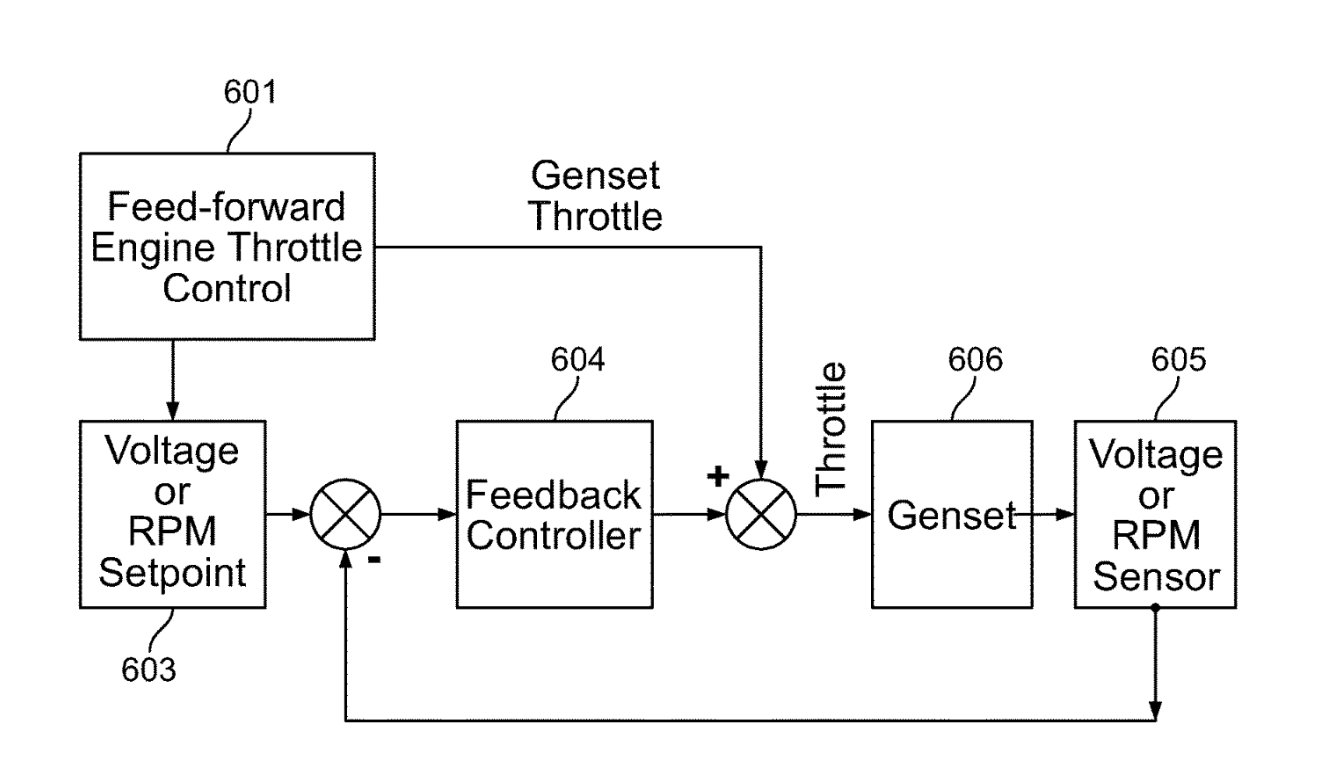
\includegraphics[scale=0.24]{patents/US10144527B2-fig6.png}
  \caption{Изображение взятое из патента US10144527B2}
\end{figure}

Полётный контроллер включает в себя, модуль управления двигателем с
обратной связью (601), источник опорного напряжения (603), контроллер
обратной связи (604), датчик напряжения или оборотов в минуту (605).

% https://patentimages.storage.googleapis.com/76/c7/4c/d47d31176792f4/US10144527.pdf

В ~\cite{TW202504822A} представлен беспилотный летательный аппарат
мультироторного типа, использующий умное устройство в качестве
полётного контроллера.

\begin{figure}[H]
  \centering
  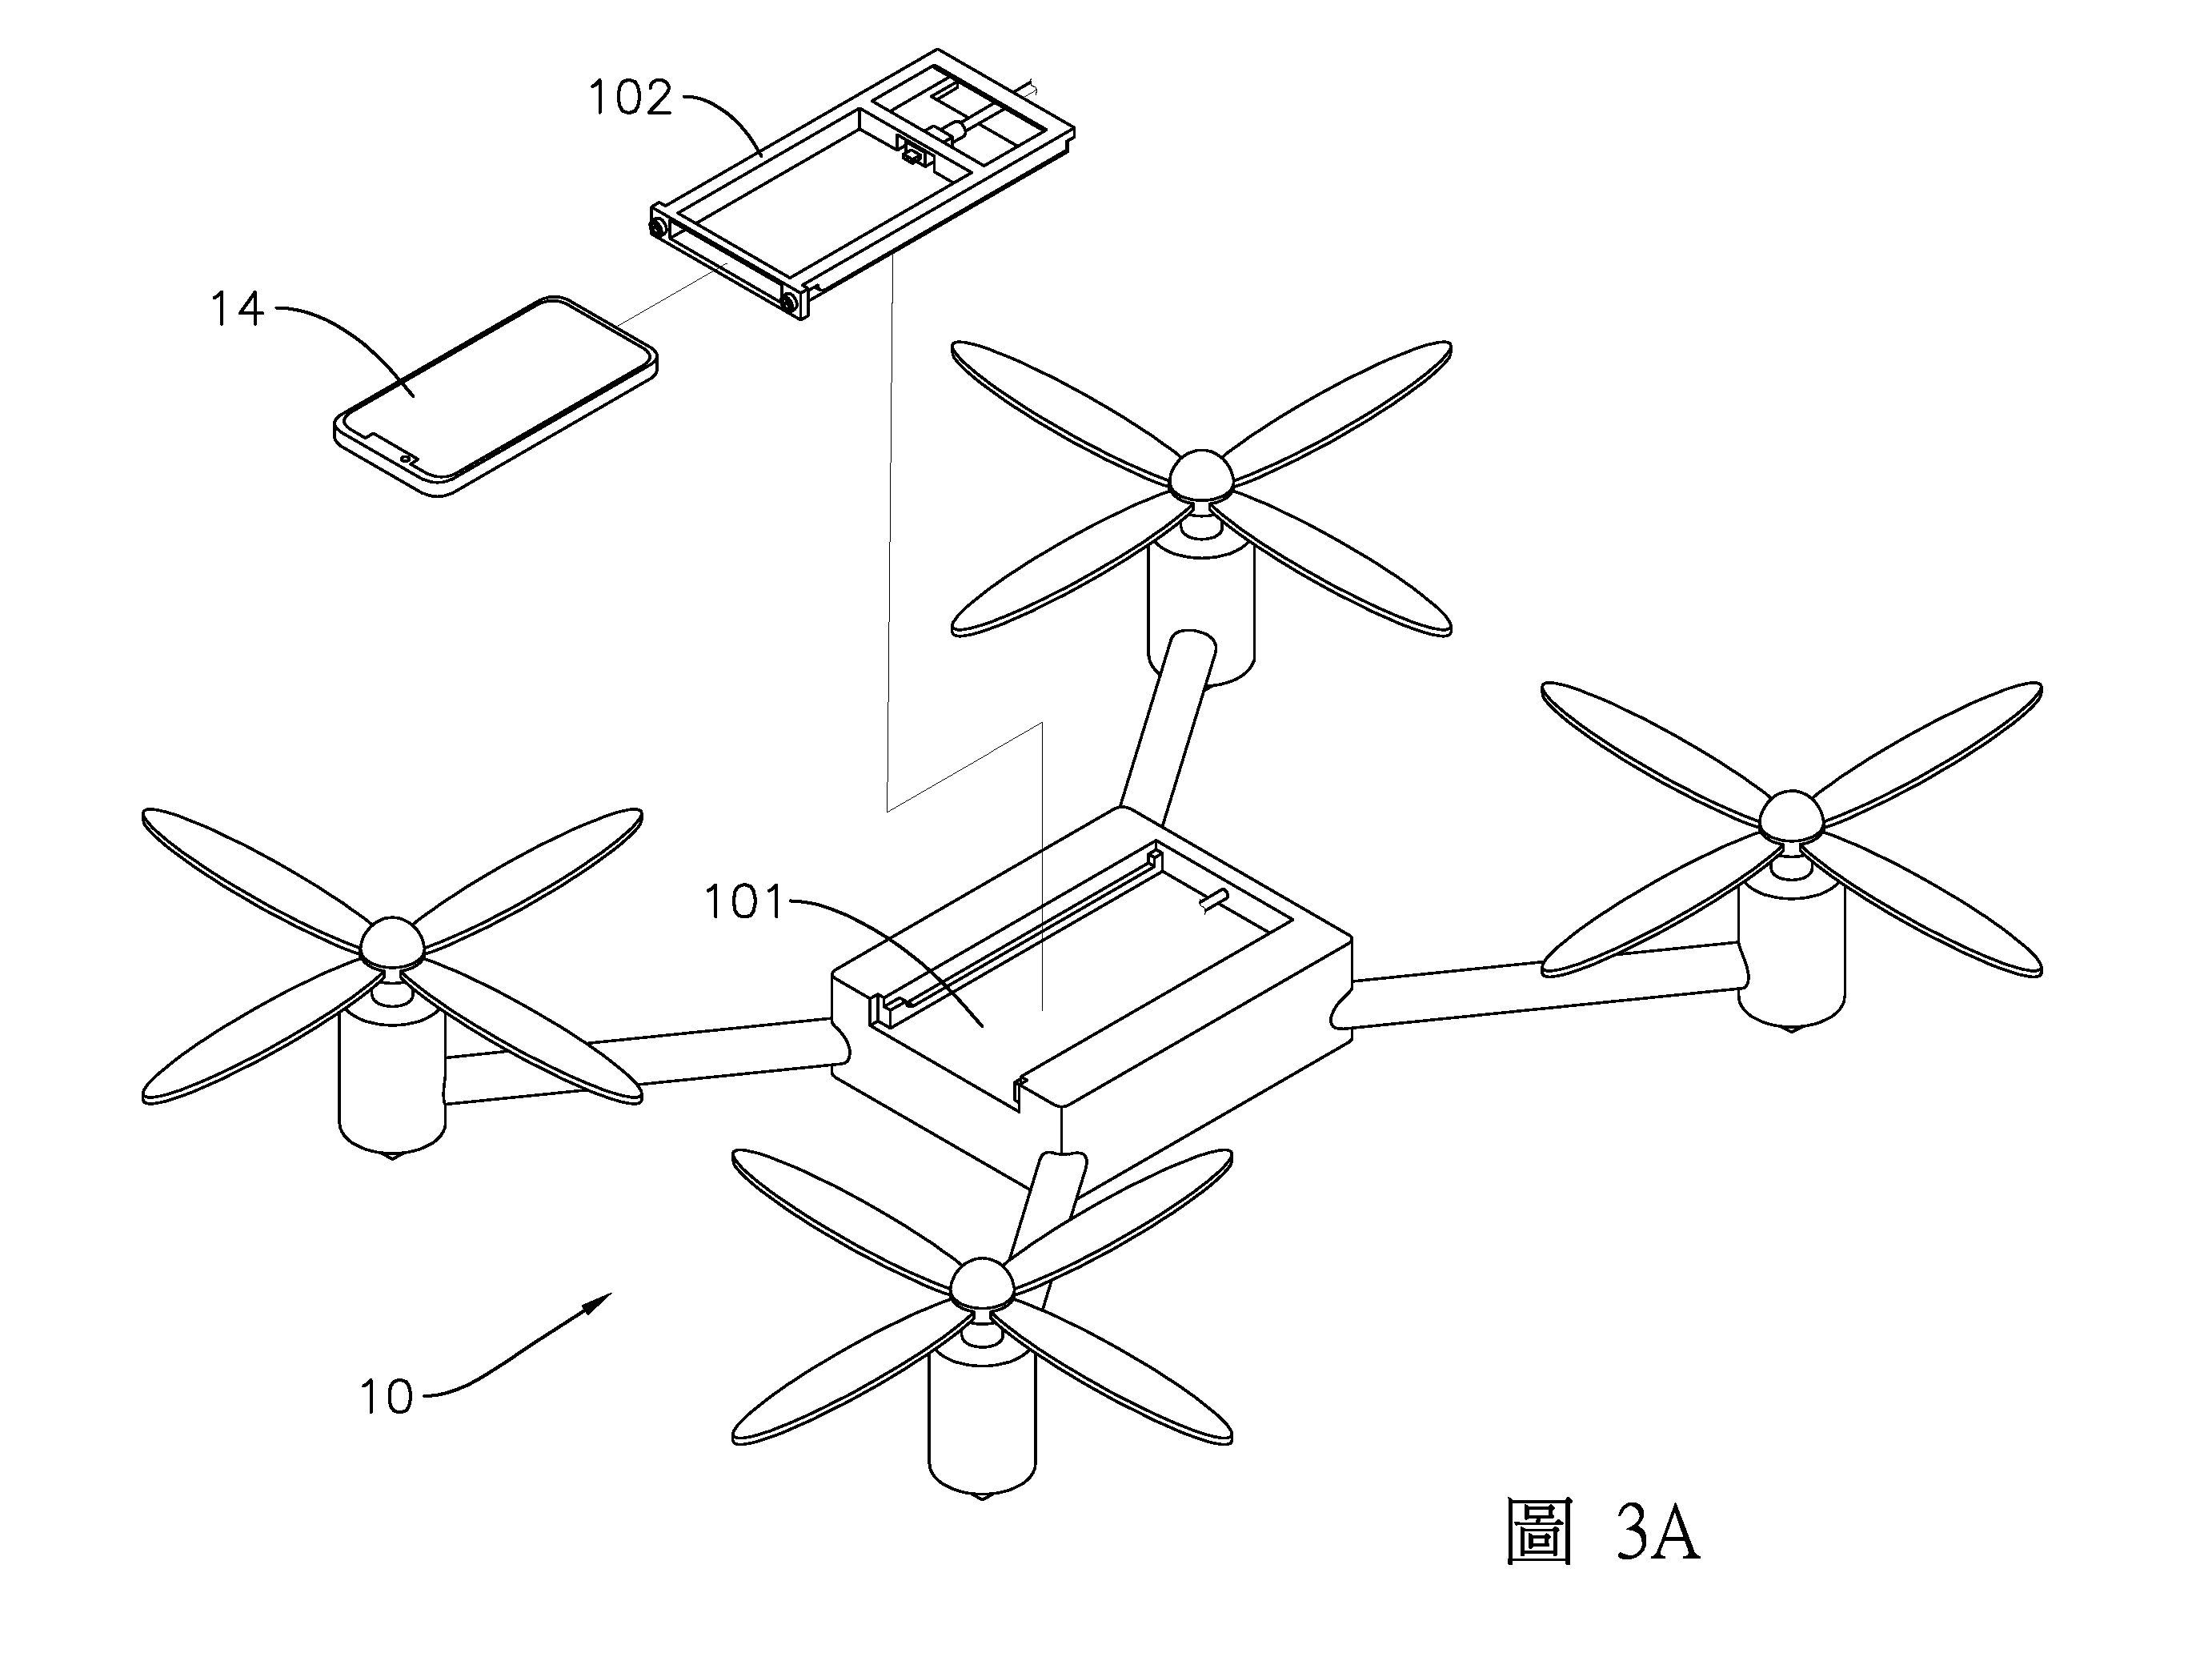
\includegraphics[scale=0.10]{patents/TW202504822A-fig4.png}
  \caption{Изображение взятое из патента TW202504822A}
\end{figure}

% https://patentimages.storage.googleapis.com/3e/92/7a/2f64a534cdc244/TW202504822A.pdf

Беспилотный летательный аппарат мультироторного типа включает в
себя фюзеляж (10), приёмный слот (101) для установки корпуса (102) для
умного устройства (14).

В ~\cite{US20210245877A1} представлен полётный контроллер с
синхронизированным алгоритмом взаимодействия между сенсорами и
актуаторами.

\begin{figure}[H]
  \centering
  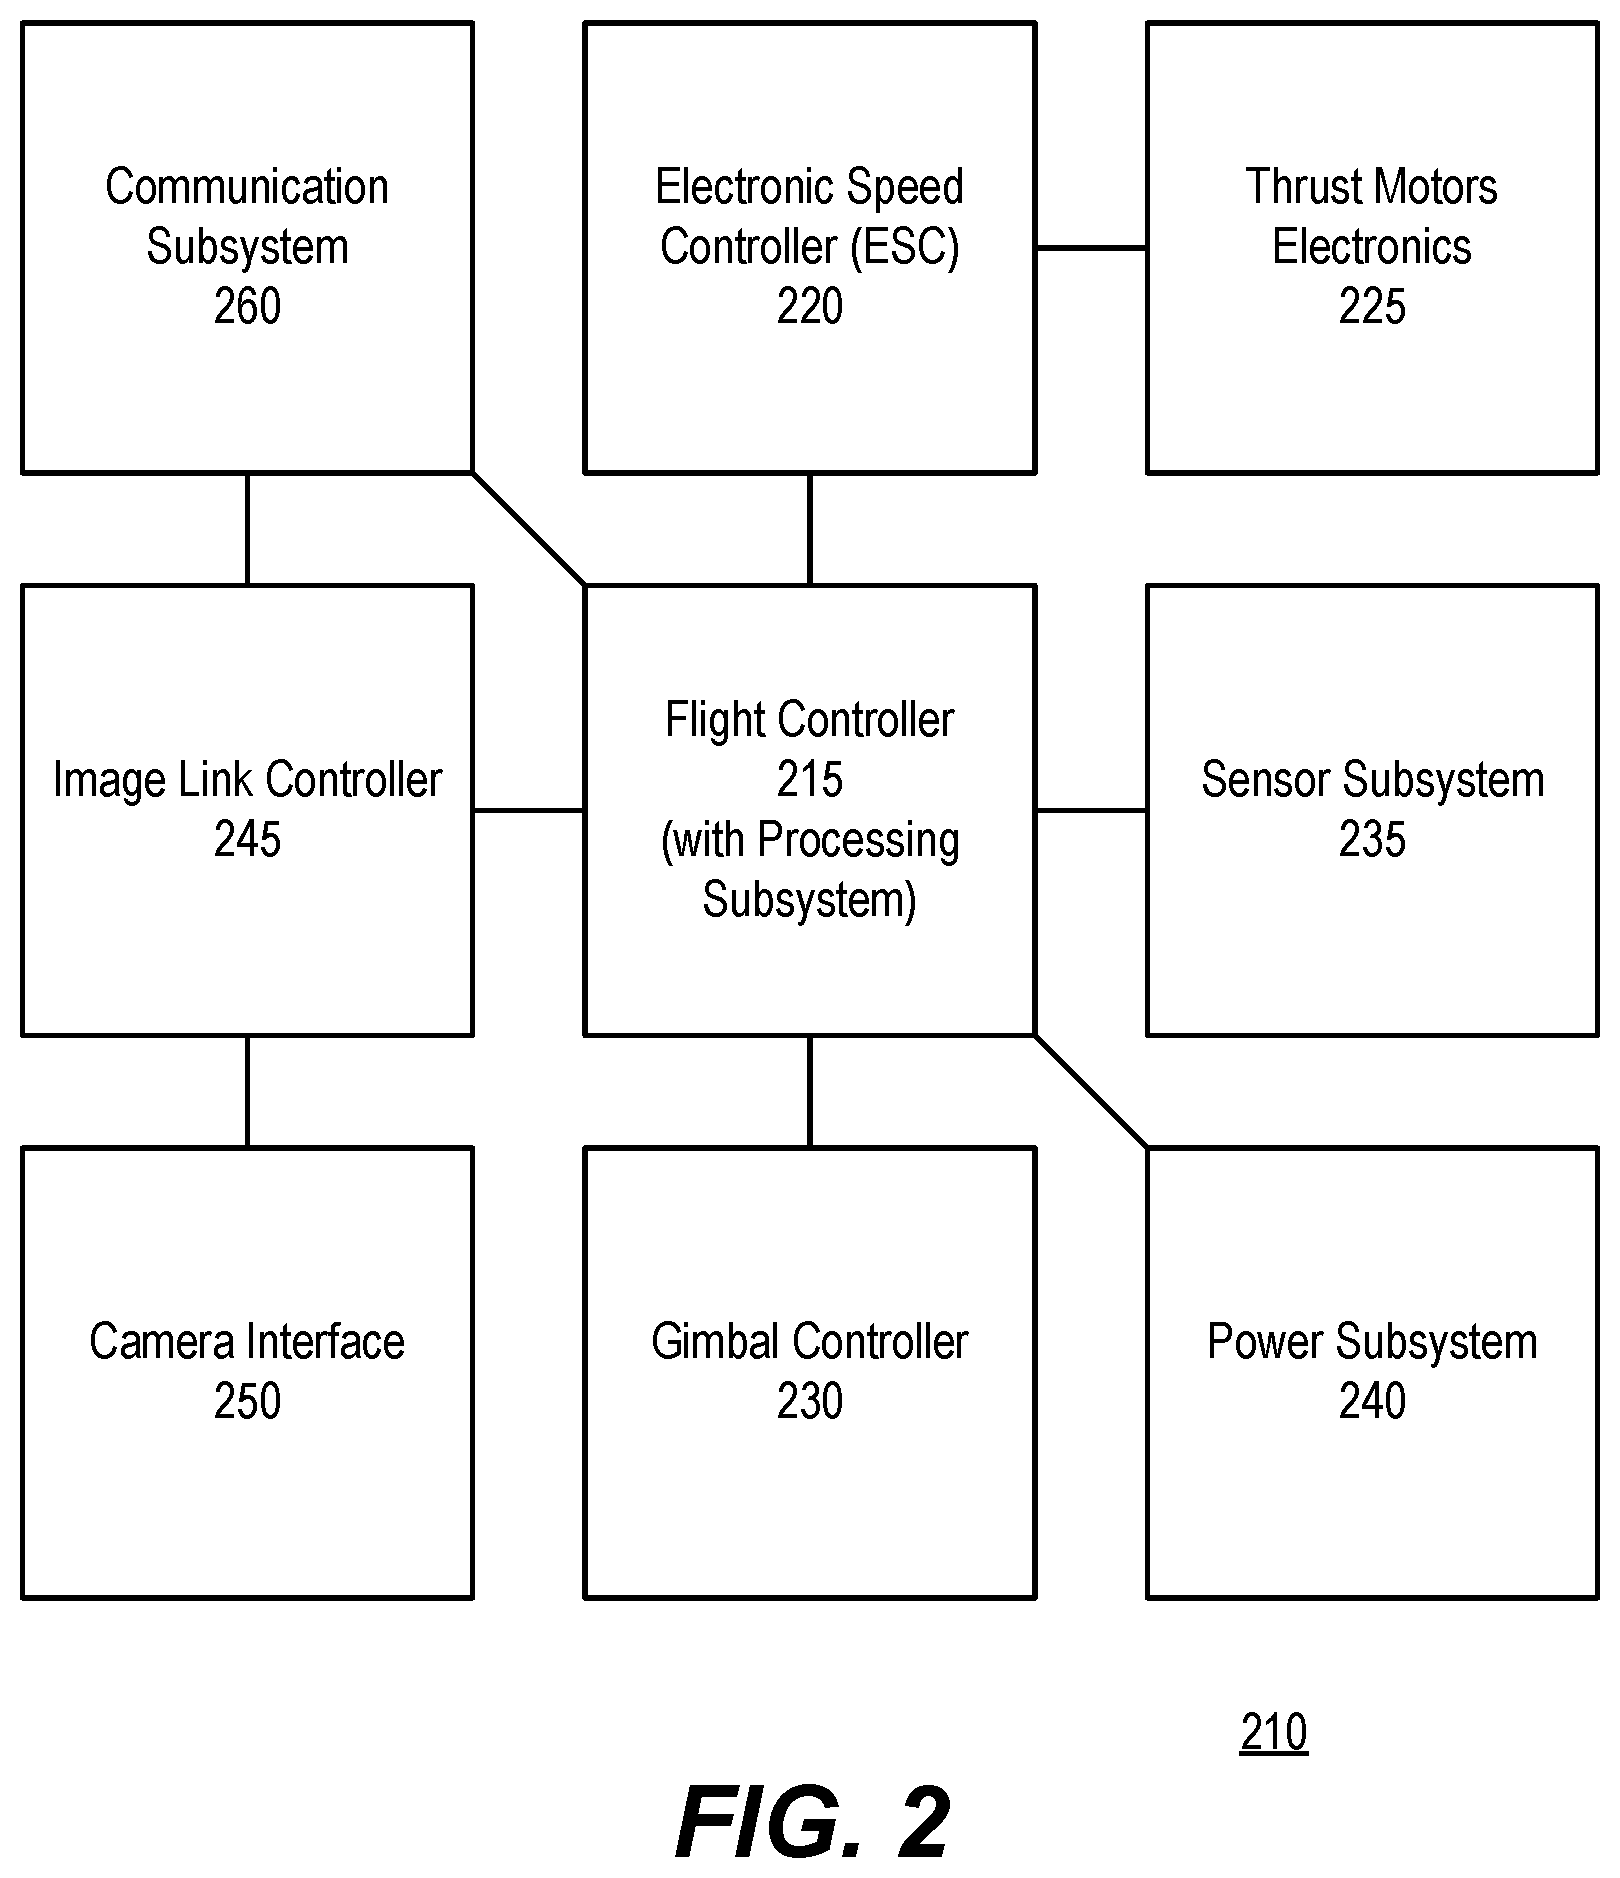
\includegraphics[scale=0.10]{patents/US20210245877A1-fig2.png}
  \caption{Изображение взятое из патента US20210245877A1}
\end{figure}

Система из беспилотного летательного аппарата мультироторного типа и
полётного контроллера(210) включает в себя полётный контроллер с
подсистемой обработки данных (215), электронный регулятор скорости
(220), электронику тяговых двигателей (225), подсистему датчиков
(235), подсистему питания (240), контроллер данных камеры (245),
интерфейс камеры (250), подсистему коммуникаций (260).

В ~\cite{US10551834B2} представлено электронное устройство для
управления беспилотном летательным аппаратом и соответствующий метод.

\begin{figure}[H]
  \centering
  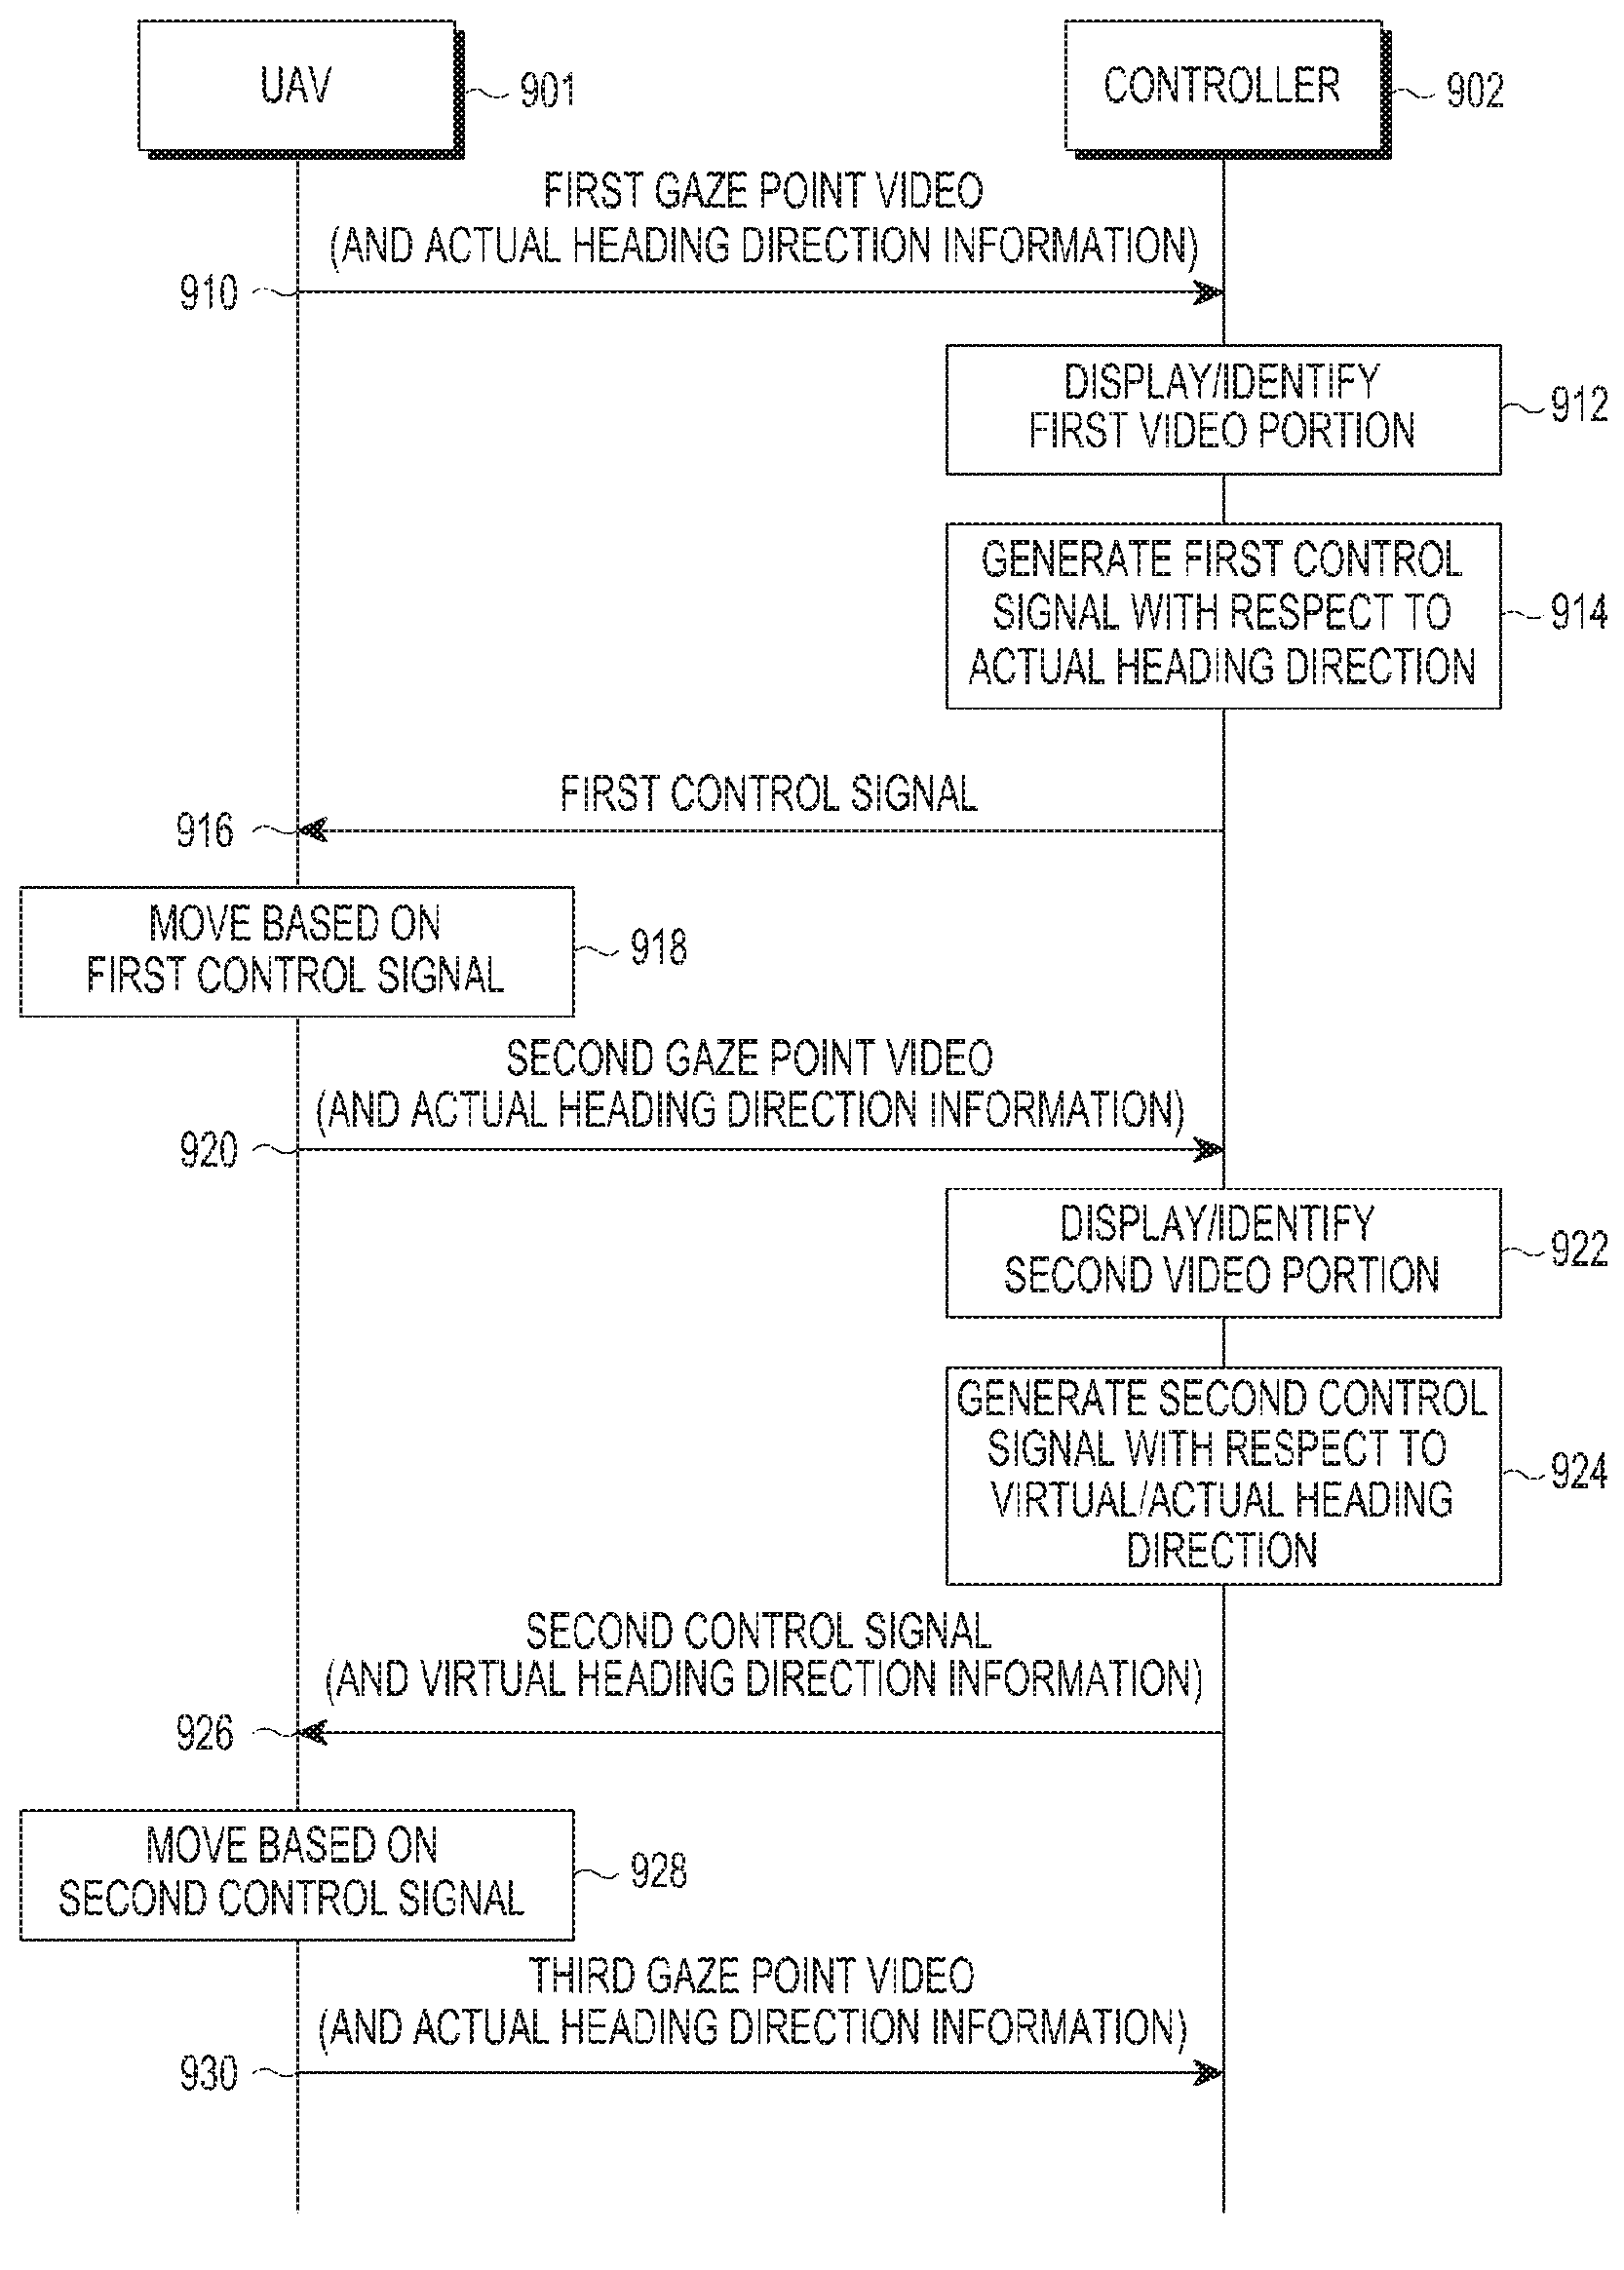
\includegraphics[scale=0.12]{patents/US10551834B2-fig9.png}
  \caption{Изображение взятое из патента US10551834B2}
\end{figure}

На рисункке 1.4 представлен алгоритм работы полётного контроллера:
Беспилотный летательный аппарат (901) отправляет видео (910) с первой
точки обзора и настоящую информацию о направлении полёта, полётный
контроллер (902) распознаёт (912) первый видеофрагмент и генерирует
(914) первый управляющий сигнал, соответствующий направлению полёта.
Первый управляющий сигнал отправляется (916) беспилотному летательному
аппарату. Беспилотный летательный аппарат приводится в движение (918)
первым управляющим сигналом.
Видеофрагмент со второй точки обзора и настоящая информация о
направлении полёта посылаются (920) беспилотным летательным аппаратом
контроллеру. Идентифицируется(922) второй видеофрагмент. Генерируется
(924) второй управляющий сигнал, соотвествующий направлению движения.
Второй управляющий сигнал посылается (926) БПЛА.
Происходит перемещение (926) в результате обработки второго сигнала.
Посылается (930) видеофрагмент с третьей точки обзора с информацией о
настоящем направлении, цикл повторяется.

В ~\cite{CN113341830A} представлен полётный контроллер для
четырёхроторного БПЛА. Описываемая система включает в себя:
\begin{enumerate}
\item Модуль питания с низким уровнем шума и восокой стабильностью.
\item Модуль микроконтроллерного устройства для анализа и обработки данных.
\item Сенсорный модуль для мониторинга условий окружающей среды.
\item Модуль хранения для записи различных данных.
\item Световой модуль для управления включением-выключением с помощью МОП (металл-оксид-полупроводник) трубки.
\item Модуль дистанционного управления.  
\item Модуль микроконтроллера, соединенный с модулем датчиков, модулем
хранения, модулем освещения и модулем дистанционного управления.
\end{enumerate}

\begin{figure}[H]
  \centering
  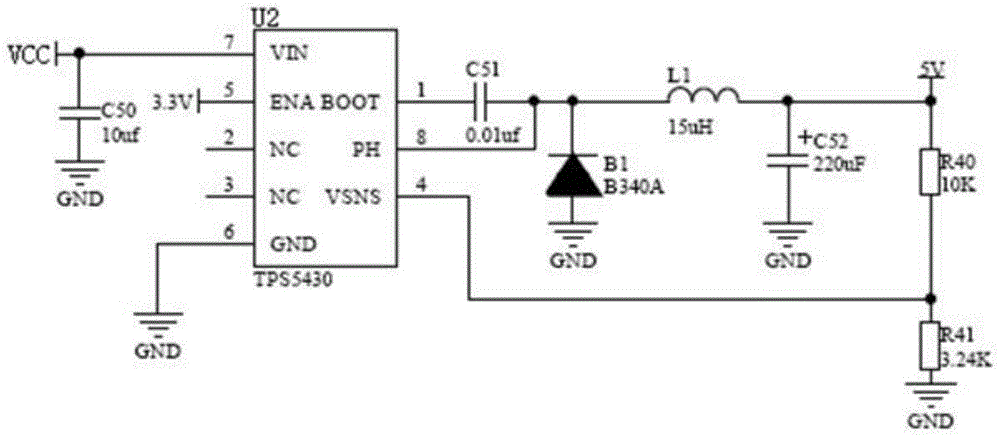
\includegraphics[scale=0.4]{patents/CN113341830A-fig2.png}
  \caption{Схема цепи питания батереи. Изображение взято из патента CN113341830A.}
\end{figure}

На рисунке 1.5 изображена схема цепи питания батареи настоящего
патента.  Согласно данной схеме цепь питания батареи состоит из
источника питания, резисторов R40-R41, кондесаторов С50-С52, дросселя
индуктивности L1, диода B1, и ИМС U2 модели TPS5430.

\begin{figure}[H]
  \centering
  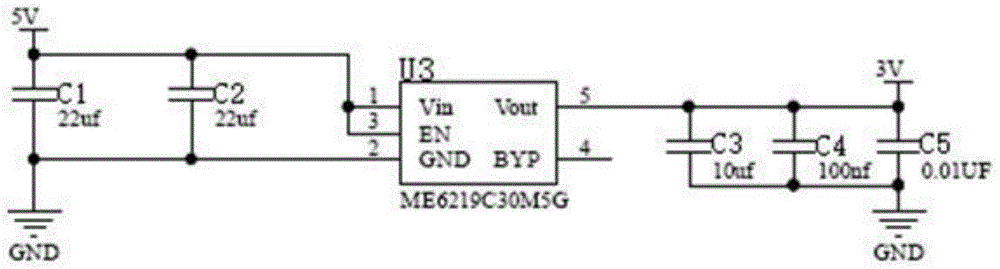
\includegraphics[scale=0.4]{patents/CN113341830A-fig3.png}
  \caption{Схема цепи питания барометра. Изображение взято из патента CN113341830A.}
\end{figure}

На рисунке 1.6 изображена схема цепи питания барометра настоящего патента.
Согласно данной схеме цепь питания состоит из конденсаторов С1-С5 и ИМС U3 модели
ME6219C30M 5G

\begin{figure}[H]
  \centering
  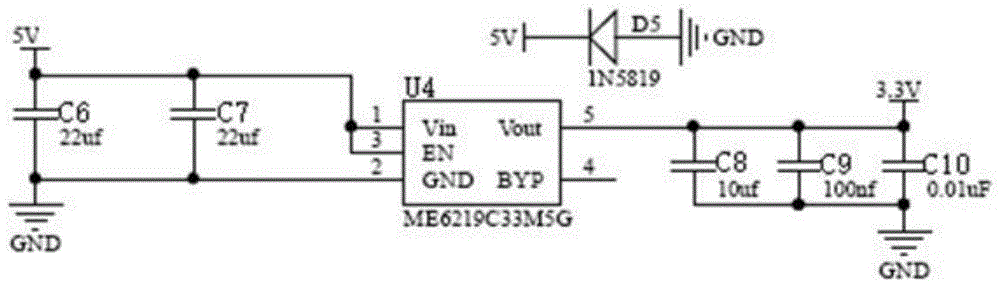
\includegraphics[scale=0.4]{patents/CN113341830A-fig4.png}
  \caption{Схема цепи питания датчика. Изображение взято из патента CN113341830A.}
\end{figure}

На рисунке 1.7 изображена схема цепи питания датчика настоящего
патента, состоящая из конденсаторов C6-C10, диода D5 и ИМС U4 модели
ME6219C33M 5G

% Если нужно будет добавить ещё воды, то можно напихать схем из этого
% патента.
Основные отличия разрабатываемой в данном работе системы заключаются в
следующем:
\begin{enumerate}
  
\item Полётнык контроллер управляет только показателями
непосредственно связанными с ШИМ сигналом подаваемом на входы
сервоприводов;
  
\item Изделие использует один только микроконтроллер и не
  подразумевает подключения к ЭВМ или использования нескольких ЭВМ или
умных устройств для вычислений;
  
\item Отсуствуют какие-либо строго оговоренные алгоритмы построения
маршрута, которые применялись бы при работе полётного контроллера.
\end{enumerate}

В заключении остаётся добавить, что найденные при патентном поиске
изделия значительно отличались от разрабатываемого в данной работе
устройства.



\newpage
%%% Local Variables:
%%% mode: LaTeX
%%% TeX-master: "main"
%%% End:
